% Created 2024-10-16 śro 21:35
% Intended LaTeX compiler: pdflatex
\documentclass[../../main.tex]{subfiles}

% \usepackage[a4paper, margin=3cm]{geometry}
% \usepackage{amssymb} // not working

\usepackage[T1]{fontenc}
\usepackage[utf8]{inputenc}
\usepackage{graphicx}
\usepackage{longtable}
\usepackage{wrapfig}
\usepackage{rotating}
\usepackage[normalem]{ulem}
\usepackage{amsmath}
\usepackage{capt-of}
\usepackage{hyperref}
\usepackage{siunitx}
\usepackage{float}
\usepackage[polish]{babel}

\graphicspath{{../}}
\author{Wojciech Paderewski}
\date{\today}
\title{Koncepcja ukladu}
\hypersetup{
 pdfauthor={Wojciech Paderewski},
 pdftitle={Koncepcja ukladu},
 pdfkeywords={},
 pdfsubject={},
 pdflang={Polish}}

\begin{document}

\subsubsection{Dobór złącza}
W doborze złącza kluczowe kluczowa była jego wielkość oraz prąd, który jest w stanie przewodzić. Teoretyczna moc układu to 10W,
co przy napięciu \SI{12}{\volt} daje prąd \SI{0.83}{\ampere}. Złącze musi być w stanie przewodzić prąd 1.5A, by zapewnić bezpieczeństwo. 

Wybrano złącze firmy Same Sky o symbolu PJ-094H-SMT-TR o styku 0.65x2.35 mm, które jest w stanie przewodzić prąd 2.5A, czyli więcej niż wystarczająco.
Złącze jest bardzo niskie, jego wysokość to 3.5mm, co pozwala na zminimalizowanie wysokości zegara.
\subsubsection{Opis podłączenia}
Jako kondensatory filtrujące wykorzystano, 2 kondensatory o 
pojemności \SI{100}{\micro\farad}  w celu zminimalizowania zakłóceń niskich częstotliwości, oraz 1 kondensator o pojemności \SI{100}{\nano\farad} w celu zminimalizowania zakłóceń wysokich częstotliwości.

Kondensatory \SI{100}{\micro\farad}  są kondensatorami tantalowymi, a kondensator \SI{100}{\nano\farad} jest kondensatorem ceramicznym. Wykorzystano te rodzaje kondensatorów, 
ponieważ są to kondensatory o długiej żywotności, a także mają one małe rozmiar w przeciwieństwie do kondensatorów elektrolitycznych.
\subsubsection{Zabezpieczenia ESD}
W celu zabezpieczenia linii przed przepięciami, wykorzystano diodę Transila firmy Wurth Elektronik o symbolu 824045812. Dioda ta jest diodą TVS o napięciu przebicia \SI{13.3}{\volt},
oraz napięciu stabilizacji \SI{15}{\volt}. Dioda musi mieć jak najmniejsze napięcie przebicia, by skok napięcia nie uszkodził rejestrów przesuwnych HV, które są wrażliwe na napięcia powyżej \SI{13.2}{\volt}.

Dioda ta została wybrana gdyż nie udało się znaleźć transila o napięciu stabilizacji \SI{13}{\volt}. Ma ona również dużą pojemność, co powoduje, że nie jest ona zalecana do 
zastosowań z wysokimi częstotliwościami, jednak w tym przypadku nie jest to problemem, gdyż jest to tylko złącze zasilania o stałym napięciu. 
Schemat złącza zasilania przedstawiono na rysunku \ref{fig:DcPlug_schemat}.
\begin{figure}[H]
    \centering
    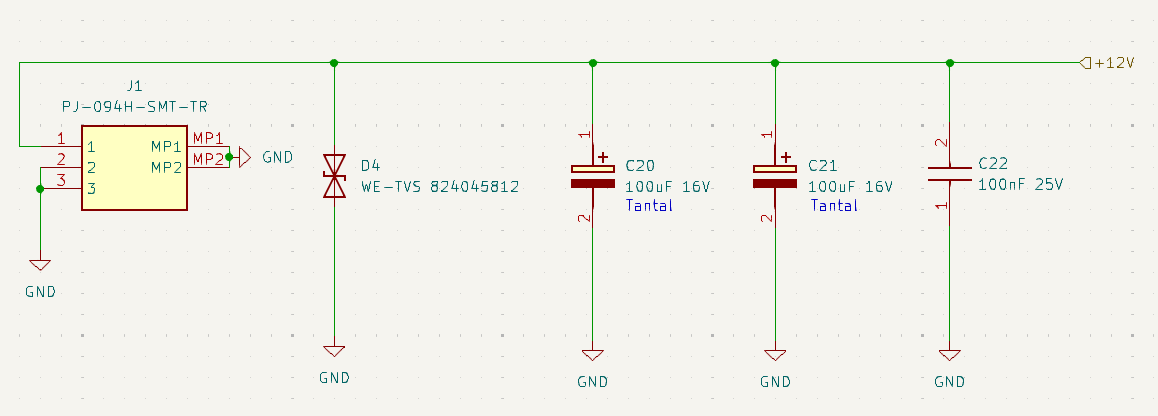
\includegraphics[width=0.8\textwidth]{dc_plug_schemat.png}
    \caption{Schemat elektryczny złącza zasilania}
    \label{fig:DcPlug_schemat}
\end{figure}

\end{document}
